%%%%%%%%%%%%%%%%%%%%%%%%%%%%%%%%%%%%%%%%%
% Short Sectioned Assignment LaTeX Template Version 1.0 (5/5/12)
% This template has been downloaded from: http://www.LaTeXTemplates.com
% Original author:  Frits Wenneker (http://www.howtotex.com)
% License: CC BY-NC-SA 3.0 (http://creativecommons.org/licenses/by-nc-sa/3.0/)
%%%%%%%%%%%%%%%%%%%%%%%%%%%%%%%%%%%%%%%%%

%----------------------------------------------------------------------------------------
%	PACKAGES AND OTHER DOCUMENT CONFIGURATIONS
%----------------------------------------------------------------------------------------

\documentclass[paper=a4, fontsize=11pt]{scrartcl} % A4 paper and 11pt font size

% ---- Entrada y salida de texto -----

\usepackage[T1]{fontenc} % Use 8-bit encoding that has 256 glyphs
\usepackage[utf8]{inputenc}

% ---- Idioma --------

\usepackage[spanish, es-tabla]{babel} % Selecciona el español para palabras introducidas automáticamente, p.ej. "septiembre" en la fecha y especifica que se use la palabra Tabla en vez de Cuadro

% ---- Otros paquetes ----

\usepackage{amsmath,amsfonts,amsthm} % Math packages
\usepackage{graphics,graphicx, floatrow} %para incluir imágenes y notas en las imágenes
\usepackage{graphics,graphicx, float} %para incluir imágenes y colocarlas
\usepackage{hyperref} % url in references

% Para hacer tablas comlejas
\usepackage{multirow}
\usepackage{threeparttable}

\usepackage{fancyhdr} % Custom headers and footers
\pagestyle{fancyplain} % Makes all pages in the document conform to the custom headers and footers
\fancyhead{} % No page header - if you want one, create it in the same way as the footers below
\fancyfoot[L]{} % Empty left footer
\fancyfoot[C]{} % Empty center footer
\fancyfoot[R]{\thepage} % Page numbering for right footer
\renewcommand{\headrulewidth}{0pt} % Remove header underlines
\renewcommand{\footrulewidth}{0pt} % Remove footer underlines
\setlength{\headheight}{13.6pt} % Customize the height of the header

\numberwithin{equation}{section} % Number equations within sections (i.e. 1.1, 1.2, 2.1, 2.2 instead of 1, 2, 3, 4)
\numberwithin{figure}{section} % Number figures within sections (i.e. 1.1, 1.2, 2.1, 2.2 instead of 1, 2, 3, 4)
\numberwithin{table}{section} % Number tables within sections (i.e. 1.1, 1.2, 2.1, 2.2 instead of 1, 2, 3, 4)

\setlength\parindent{0pt} % Removes all indentation from paragraphs - comment this line for an assignment with lots of text

\newcommand{\horrule}[1]{\rule{\linewidth}{#1}} % Create horizontal rule command with 1 argument of height
\usepackage{textcomp}
\usepackage{listings}
\usepackage{color}

\definecolor{mygreen}{rgb}{0,0.6,0}
\definecolor{mygray}{rgb}{0.5,0.5,0.5}
\definecolor{mymauve}{rgb}{0.58,0,0.82}

\lstset{ %
  backgroundcolor=\color{white},   % choose the background color; you must add \usepackage{color} or \usepackage{xcolor}; should come as last argument
  breakatwhitespace=false,         % sets if automatic breaks should only happen at whitespace
  breaklines=true,                 % sets automatic line breaking
  captionpos=b,                    % sets the caption-position to bottom
  commentstyle=\color{mygreen},    % comment style
  deletekeywords={...},            % if you want to delete keywords from the given language
  escapeinside={\%*}{*)},          % if you want to add LaTeX within your code
  extendedchars=true,              % lets you use non-ASCII characters; for 8-bits encodings only, does not work with UTF-8
  frame=single,	                   % adds a frame around the code
  keepspaces=true,                 % keeps spaces in text, useful for keeping indentation of code (possibly needs columns=flexible)
  keywordstyle=\color{blue},       % keyword style
  language=C,                 % the language of the code
  morekeywords={*,...},            % if you want to add more keywords to the set
  numbers=left,                    % where to put the line-numbers; possible values are (none, left, right)
  numbersep=5pt,                   % how far the line-numbers are from the code
  numberstyle=\tiny\color{mygray}, % the style that is used for the line-numbers
  rulecolor=\color{black},         % if not set, the frame-color may be changed on line-breaks within not-black text (e.g. comments (green here))
  showspaces=false,                % show spaces everywhere adding particular underscores; it overrides 'showstringspaces'
  showstringspaces=false,          % underline spaces within strings only
  showtabs=false,                  % show tabs within strings adding particular underscores
  stringstyle=\color{mymauve},     % string literal style
  tabsize=2,	                   % sets default tabsize to 2 spaces
}

\usepackage[table,xcdraw]{xcolor}


\newpage         


%----------------------------------------------------------------------------------------
%	INDICE
%----------------------------------------------------------------------------------------

\begin{document}
	
\setcounter{page}{0}

\begin{titlepage}
 
 
\newlength{\centeroffset}
\setlength{\centeroffset}{-0.5\oddsidemargin}
\addtolength{\centeroffset}{0.5\evensidemargin}
\thispagestyle{empty}

\noindent\hspace*{\centeroffset}\begin{minipage}{\textwidth}

\centering

\includegraphics[width=0.9\textwidth]{images/logo_ugr.jpg}\\[1.4cm]

\textsc{ \Large CLOUD COMPUTING: SERVICIOS Y APLICACIONES\\[0.2cm]}
\textsc{ MÁSTER EN INGENIERÍA INFORMÁTICA }\\[1cm]
% Upper part of the page
% 
% Title
{\Huge\bfseries Computación	Distribuida	y	Escalable	con	Hadoop	}
\noindent\rule[-1ex]{\textwidth}{3pt}\\[3.5ex]
{\large\bfseries Práctica 4}
\end{minipage}

\vspace{4.5cm}
\noindent\hspace*{\centeroffset}\begin{minipage}{\textwidth}
\centering

\textbf{Autor}\\ {Juan Pablo Porcel Porcel - juanpiporcel@correo.ugr.es}\\[1cm]

\includegraphics[width=0.3\textwidth]{images/etsiit_logo.png}\\[0.1cm]
\textsc{Escuela Técnica Superior de Ingenierías Informática y de Telecomunicación}\\
\textsc{---}\\
Granada, 22 de mayo de 2017
\end{minipage}
%\addtolength{\textwidth}{\centeroffset}
%\vspace{\stretch{2}}
\end{titlepage}




\thispagestyle{empty}

\newpage %inserta un salto de página

\tableofcontents % para generar el índice de contenidos

%\listoffigures

\newpage

%----------------------------------------------------------------------------------------
%	DOCUMENTO
%----------------------------------------------------------------------------------------

\section{Introducción}

El objetivo de esta práctica es familiarizarse con el uso de una plataforma IaaS y desarrollar habilidades de despliegue de máquinas virtuales y aplicaciones web sencillas.

Para ello el alumno deberá realizar las siguientes tareas:

\begin{itemize}
	\item Crear dos máquinas virtuales, cada una con una distribución Linux.
	\begin{enumerate}
		\item En la primera máquina instalará y configurará un servidor web.
		\item En la segunda instalará y configurará un Sistema de Gestión de Base de Datos.
	\end{enumerate}
	\item Desarrollar una aplicación web sencilla alojada en la primera máquina, que use una base de datos manejada por el SGBD instalado en la segunda. La aplicación web debe incluir el uso de formularios y la consulta y modificación de datos almacenados en la base de datos.
	\item Realizar el despliegue de ambas máquinas virtuales para evaluar el funcionamiento de la aplicación.
	\item Elaborar un breve documento detallando el trabajo realizado.

\end{itemize}


\section{Configuración de las máquinas virtuales}

Para esta práctica se han desplegado y configurado dos máquinas virtuales sobre el IaaS OpenNebula que se describen a continuación. En la Figura \ref{fig:ccsa} se puede ver la conexión entre ambas máquinas.

\begin{figure}[h!]
	\centering
	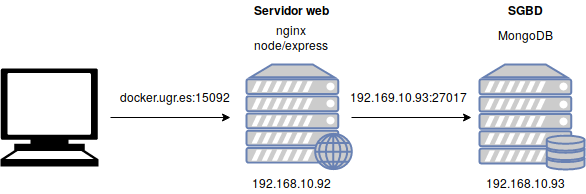
\includegraphics[width=13cm]{./images/ccsa}
	\caption{Conexión entre las máquinas virtuales y el exterior.} 
	\label{fig:ccsa}
\end{figure}


\subsection{SGBD}

La primera máquina que debemos de levantar será la que alojará la base de datos para que cuando levantemos la segunda máquina y despleguemos el servicio web no tengamos problemas para conectarnos a la base de datos. \\

Para esta máquina virtual se ha usado la siguiente plantilla: \\

\begin{lstlisting}
onetemplate create --name "DB_centos7" --cpu 1 --vcpu 1 --memory 512 
--arch x86_64 --disk 9 --nic 225 --vnc --ssh --net_context
\end{lstlisting}

Donde se especifican el número de cpus, la memoria asignada, arquitectura, imagen y red virtual (--nic 225). Para esta máquina virtual se ha optado por una imagen CentOS 7 (--disk 9). \\

Ahora podemos instanciar esta plantilla con \textbf{onetemplate instantiate <id template>} para que OpenNebula cree una nueva máquina virtual con la especificación de nuestra plantilla. Una vez instanciada podemos ver el estado de la máquina virtual con: \\

\begin{lstlisting}
onevm list
\end{lstlisting}

Podemos ver la ip asignada a la máquina virtual para conectarnos a ella con: \\

\begin{lstlisting}
onevm show <id vm>
\end{lstlisting}

Una vez que alcance el estado running podemos conectarnos por ssh a la máquina virtual en la IP 192.168.10.92: \\

\begin{lstlisting}
ssh root@192.168.10.92
\end{lstlisting}

En esta máquina virtual instalaremos distintos paquetes que serán necesarios para el provisionamiento de la máquina, principalmente ansible y git. Ansible es un sistema de gestión remota de configuración que permite gestionar simultáneamente miles de sistemas diferentes. Está basado en YAML para la descripción de los sistemas y escrito en Python. Mediante Ansible crearemos una receta o playbook donde describiremos los pasos para provisionar y desplegar la aplicación. \\

\begin{lstlisting}
sudo yum install epel-release && sudo yum install ansible
\end{lstlisting}

También necesitaremos git para descargar el repositorio con el código del proyecto que se encuentra alojado en \href{https://github.com/JPPorcel/CCSA.git}. Con la siguiente orden instalamos git y clonamos el repositorio en la máquina virtual: \\

\begin{lstlisting}
sudo yum install git && git clone https://github.com/JPPorcel/CCSA.git
\end{lstlisting}

Y ejecutamos ansible pasándole como parámetro el playbook de la máquina virtual \textbf{playbook\_db.yml}. \\

\begin{lstlisting}
cd CCSA/provision/ && ansible-playbook -i "localhost," -c local playbook_db.yml
\end{lstlisting}

El contenido de este playbook se detalla en la Sección Provisionamiento. \\

El último paso que debemos de realizar es permitir las conexiones externas a la base de datos mongo. En el archivo /etc/mongod.conf debemos de cambiar el parámetro de bindIp a 0.0.0.0 de tal manera que permitamos las conexiones externas a la base de datos: \\

\begin{lstlisting}
bindIp: 127.0.0.1 --> bindIp: 0.0.0.0
\end{lstlisting}

Y reiniciamos el servicio de mongo con: \\

\begin{lstlisting}
sudo systemctl restart mongod
\end{lstlisting}

\subsection{Servidor Web}

Al igual que en la primera máquina necesitamos una plantilla para crear la nueva máquina virtual: \\

\begin{lstlisting}
onetemplate create --name "WebService_ubuntu" --cpu 1 --vcpu 1 --memory 1024 --arch x86_64 --disk 10 --nic 225 --vnc --ssh --net_context
\end{lstlisting}

Trabajaremos con Ubuntu por familiaridad con el sistema operativo, el id de la imagen con Ubuntu 14.04 es 10 (--disk 10). \\

La instanciamos y esperamos a que esté en el estado de running. Una vez que estamos dentro de la máquina instalaremos ansible y git para provisionar la máquina y clonar el repositorio respectivamente. \\

\begin{lstlisting}
sudo apt-add-repository ppa:ansible/ansible
sudo apt-get update
sudo apt-get install ansible
sudo apt install git && git clone https://github.com/JPPorcel/CCSA.git
\end{lstlisting}

Y una vez tengamos el repositorio con los fuentes y demás archivos necesarios podemos ejecutar Ansible para provisionar y desplegar el servicio web: \\

\begin{lstlisting}
cd CCSA/provision/ && ansible-playbook -i "localhost," -c local playbook.yml
\end{lstlisting}

El contenido del fichero playbook.yml se detalla en la Sección Provisionamiento. \\

\section{Aplicación web}

Una vez se hayan provisionado y desplegado las dos máquinas con Ansible la aplicación está disponible en el puerto asginado en la dirección \url{docker.ugr.es}. En nuestro caso, a la máquina que contiene el servidor web se tiene acceso por el puerto 15092. En la Figura \ref{fig:app} se puede ver una captura del servidor corriendo en la dirección \url{docker.ugr.es:15092}. \\

\begin{figure}[h!]
	\centering
	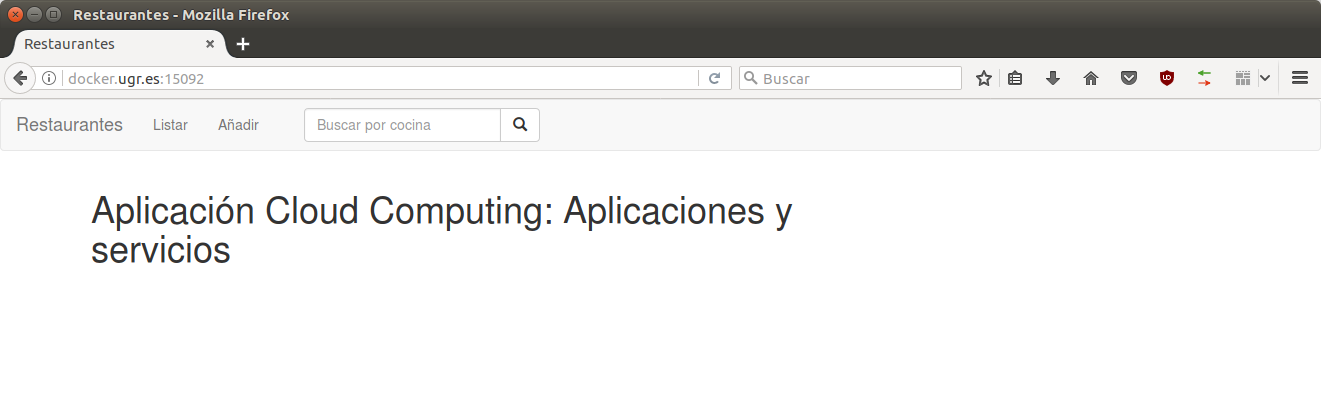
\includegraphics[width=13cm]{./images/app}
	\caption{Aplicación web corriendo en docker.ugr.es:15092} 
	\label{fig:app}
\end{figure}

La aplicación está escrita en NodeJS con Express y Pug y usa una base de datos Mongo para almacenar la información. Es una aplicación muy sencilla, se trata de un gestor de restaurantes donde se pueden añadir nuevos restaurante desde la opción de añadir que nos mostrará un formulario como el de la Figura \ref{fig:nuevo}. \\

\begin{figure}[h!]
	\centering
	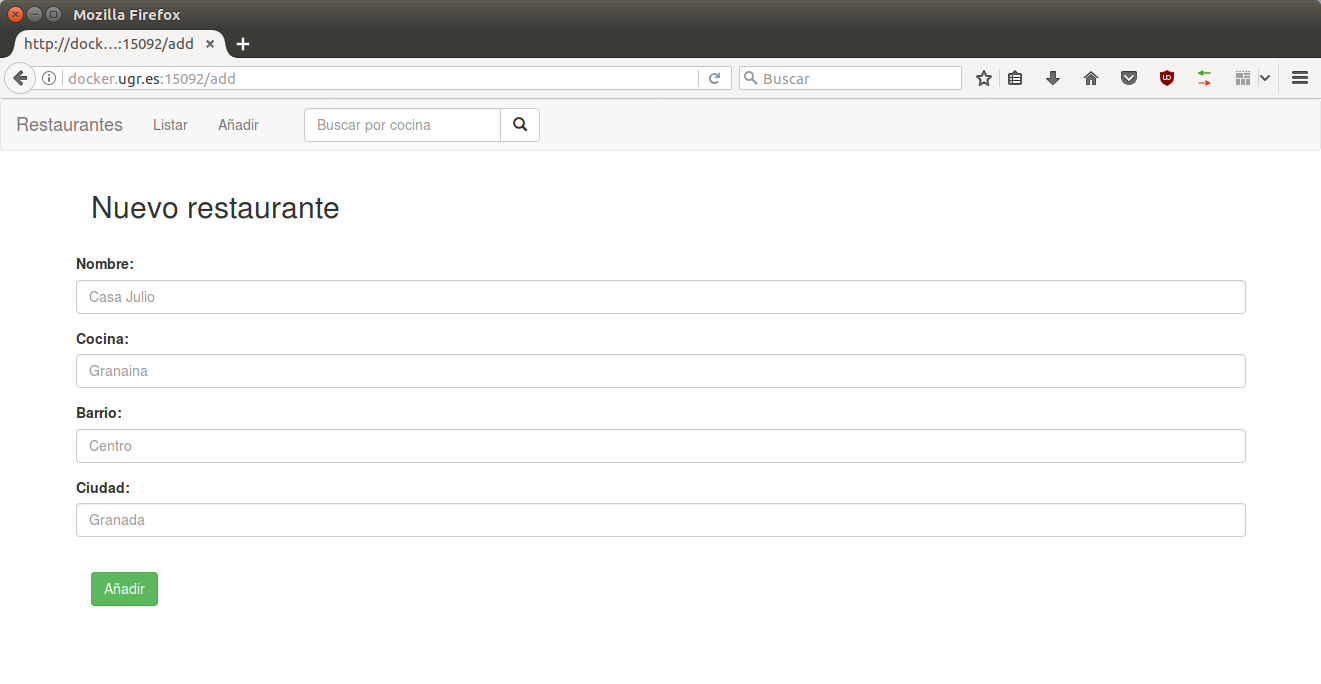
\includegraphics[width=13cm]{./images/nuevo}
	\caption{Formulario para añadir un nuevo restaurante} 
	\label{fig:nuevo}
\end{figure}

En la sección de Listar nos aparecen los primeros 20 restaurantes de la base de datos. Podemos filtrar los restaurantes por nombre, ciudad o tipo de cocina. El buscador que se encuentra implementado en la página buscará por tipo de cocina pero se pueden añadir más parámetros en la url, por ejemplo \textit{cocina=Granaina\&nombre=Julio\&ciudad=Granada}. En las Figura \ref{fig:buscar} y Figura \ref{fig:consultar} vemos la búsqueda y consulta de un restaurante añadido a la base de datos. \\

\begin{figure}[h!]
	\centering
	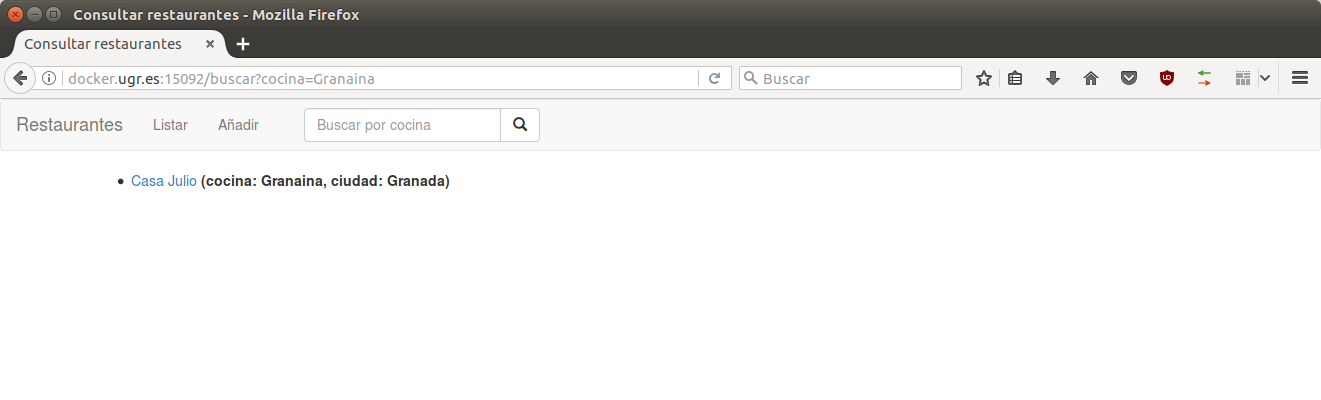
\includegraphics[width=13cm]{./images/buscar}
	\caption{Buscar un restaurante} 
	\label{fig:buscar}
\end{figure}

\begin{figure}[h!]
	\centering
	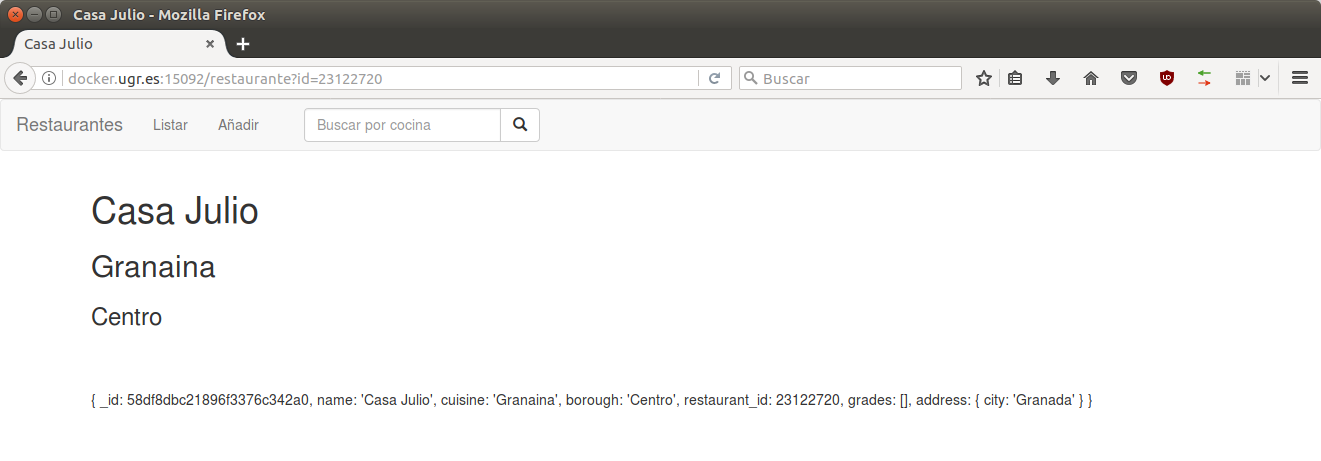
\includegraphics[width=13cm]{./images/consultar}
	\caption{Consultar un restaurante} 
	\label{fig:consultar}
\end{figure}

Es necesario cambiar en el código la dirección IP en la que se encuentra el SGBD y al que tiene acceso el servidor web. En la línea 9 del fichero server.js se encuentra la IP de la máquina que contiene la base de datos mongo. \\

\begin{lstlisting}
var express = require("express"),  
    app = express(),
    bodyParser  = require("body-parser"),
    methodOverride = require("method-override"),
    mongoose = require('mongoose');
	
	
// // Connection to DB
mongoose.connect('mongodb://192.168.10.93:27017/restaurants', function(err, res) {
  if(err) throw err;
  console.log('Connected to Database');
});
\end{lstlisting}

\section{Provisionamiento}

El fichero \textbf{playbook.yml} que se encuentra en \url{https://github.com/JPPorcel/CCSA/blob/master/provision/playbook.yml} es el encargado de provisionar y desplegar la aplicación web. \\

\begin{lstlisting}
---
- hosts: all
  sudo: yes
  
  tasks:
    - name: Update Apt cache
      apt: update_cache=yes
    
    - name: Install git
      apt: pkg=git state=present

    - name: Install NodeJS and npm
      apt: name={{ item }} state=present
      with_items:
        - nodejs
        - nodejs-dev
        - nodejs-legacy
        - npm
    
    - name: Install pm2 for manage our nodejs application
      npm:
        name: pm2
        global: yes
    
    - name: Clone repo
      git: repo=https://github.com/JPPorcel/CCSA.git dest=/opt/app version=HEAD
      
    - name: Install dependencies with npm
      shell: "cd /opt/app && sudo npm install"
      
    - name: Run server with pm2
      shell: 'cd /opt/app && pm2 start server.js && pm2 startup'
      
    - name: Install nginx
      apt: pkg=nginx state=present
      
    - name: Configure nginx
	  shell: 'cd /opt/app/provision && cp sites-available_default /etc/nginx/sites-available/default && sudo service nginx restart'
\end{lstlisting}

Ejecutando este playbook con ansible en la máquina virtual nos instalará las herramientas y paquetes necesarios para desplegar la aplicación correctamente: \\

\begin{itemize}
	\item \textbf{git}: para clonar el respositorio con el código de la aplicación.
	\item \textbf{nodejs}: para ejecutar la aplicación.
	\item \textbf{npm}: para instalar los paquetes necesarios de node especificados en el archivo package.json (\url{https://github.com/JPPorcel/CCSA/blob/master/package.json}).
	\item \textbf{pm2}: para gestionar la aplicación escrita en node.
	\item \textbf{nginx}: que sirve como servidor web y redirige las peticiones en el puerto 80 a la aplicación node en el puerto 8080.
\end{itemize}

Ansible además de instalar el software necesario desplegará la aplicación, ejecutando pm2 con nuestra aplicación y el servidor nginx. \\

De la misma manera, el fichero \textbf{playbook\_db.yml} que se encuentra en \url{https://github.com/JPPorcel/CCSA/blob/master/provision/playbook\_db.yml} es el encargado de provisionar y desplegar el SGBD. \\

\begin{lstlisting}
---
- hosts: all
  sudo: yes
  
  tasks:
    - name: Install git
      yum: name=git state=present
    
    - name: Clone repo
      git: repo=https://github.com/JPPorcel/CCSA.git dest=/opt/app version=HEAD
      
    - name: Install mongo repository
      shell: 'cd /opt/app/provision/ && cp mongodb-org.repo /etc/yum.repos.d/ && yum repolist'
      
    - name: Install mongo
      yum: name=mongodb-org state=present
      
    - name: Start mongod
      shell: 'sudo systemctl start mongod'

    - name: Load database
      shell: "cd /opt/app/mongo && mongoimport --db restaurants --collection restaurants --drop --file restaurantes.json"
      
    - name: Open ports for mongo
	  shell: 'iptables -I INPUT -p udp -m udp --dport 27017 -j ACCEPT && iptables -I INPUT -p tcp -m tcp --dport 27017 -j ACCEPT'
\end{lstlisting}

Mediante este playbook, ansible instalará mongo en la máquina CentOS, importará la base de datos que se encuentra en el repositorio y abrirá los puertos necesarios para que el servidor web pueda acceder a la base de datos mongo. \\

\section{Conclusiones}

Mediante esta práctica se ha intentado familiarizar al alumno con el uso de una plataforma IaaS. Hay algunos aspectos que se han realizado bien por parte de los responsables de la asignatura pero otros no tanto. En primer lugar, ha sido una buena elección el usar OpenNebula para realizar las prácticas ya que se trata de software libre y parece una plataforma robusta y fácil de usar. \\

Por otra parte, los problemas que nos han surgido a todos los compañeros nos han impedido realizar la práctica cómodamente. Estos problemas no han estado en la parte del cliente, nosotros, si no en la del servidor. La plataforma no respetaba el estado de las máquinas virtuales, apagándolas y reiniciándolas sin previo aviso. Además como me ha pasado a mi y a muchos compañeros, en algunos momentos, extrañamente, nuestras máquinas cambiaban a un estado pasado y perdíamos todo el trabajo realizado hasta el momento. \\



\end{document}
